\chapter{Network Layer}

\section{Network Layer}
\begin{center}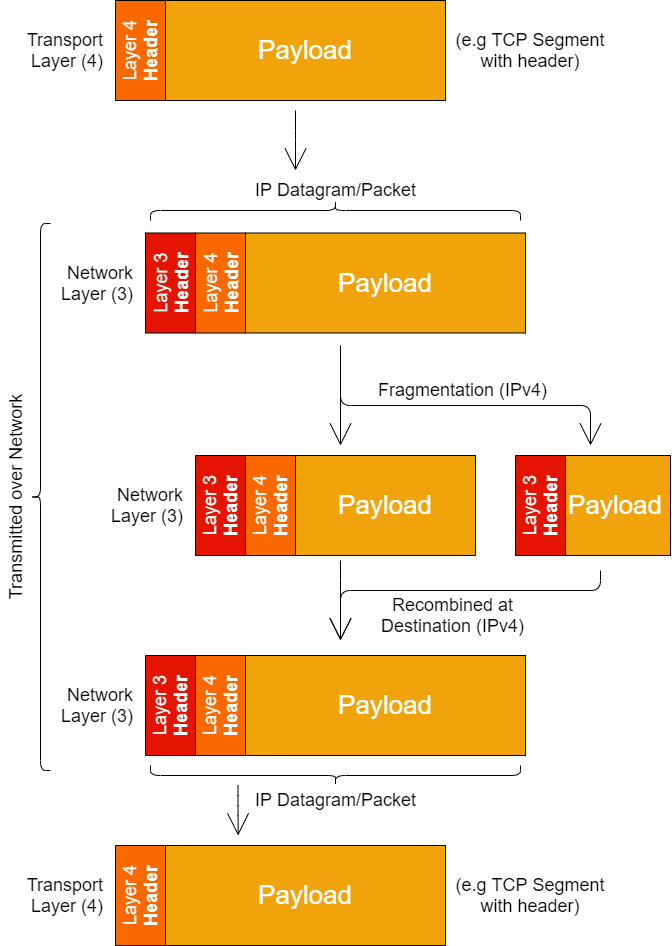
\includegraphics[width=0.8\textwidth]{network_layer/images/network layer.png}\end{center}
The network layer contains the \textbf{Internet Protocol} and is responsible for routing packets though the internet, and across networks with differing hardware, protocol stacks.
\termdef{(IP) Internet Protocol}{
    The main protocol use for this layer.
    \compitem{
        \item Datagram Format
        \item Fragmentation (IPv4 only)
        \item IP addressing
        \item Packet handling
    }
    \begin{center}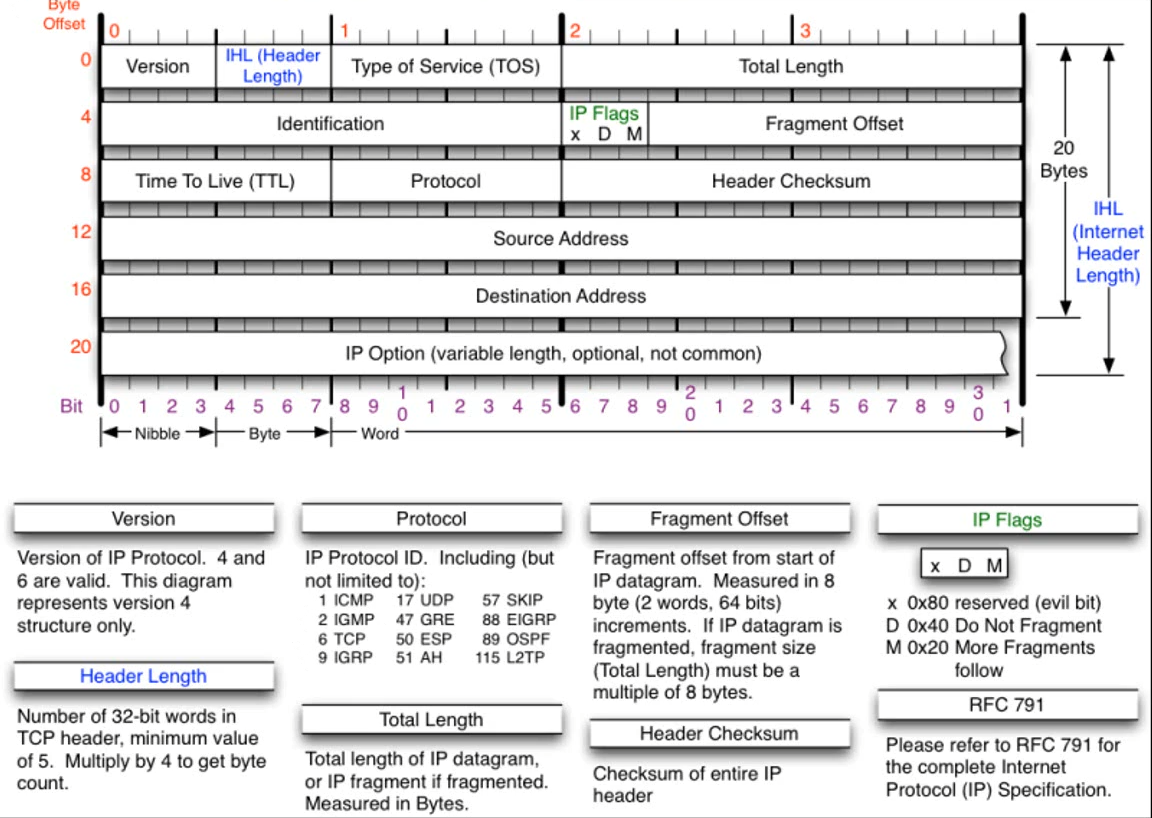
\includegraphics[width=0.8\textwidth]{network_layer/images/IP Header.png}\end{center}
    Note that:
    \compitem{
        \item Type of Service is now called \textbf{DiffServ}.
        \item Most IP Options are not used (security issues).
    }
}
\termdef{Fragmentation}{
    \begin{center}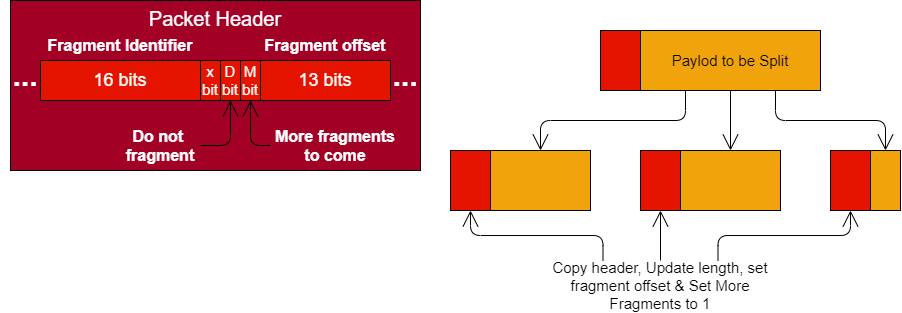
\includegraphics[width=0.7\textwidth]{network_layer/images/fragmentation.png}\end{center}
    When the data sent to \textbf{IPv4} is larger than the \textbf{MTU} (maximum transmission unit) of the output link it is being forwarded through the \textbf{IP datagram} needs to be split (fragmented).
    \compitem{
        \item Fragmentation at the start, or any intermediate routers.
        \item Only reassembled at the destination.
        \item Each fragment is identified by its 16-bit \textbf{fragment identifier}.
        \item Each fragment offset is the offset in units of 8-bytes (all fragments will be multiples of 8 bytes, plus a last byte).
        \item The \textbf{more fragments} bit (\textbf{M}) informs the receiver if it should expect more fragments to arrive, this is set when an intermediate router fragments a packet.
    }
}
\sidenote{Maximum Fragments}{
    It is not possible to fit the maximum number of fragments allowed by the 13-Bit fragment offset ($8192$) inside an \textbf{IP Datagram}/\textbf{Packet}.
    \begin{center}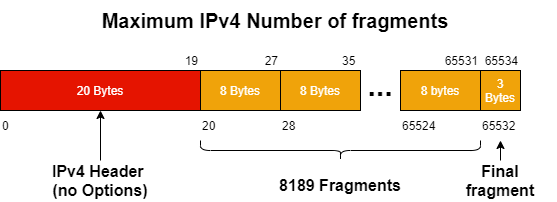
\includegraphics[width=0.7\textwidth]{network_layer/images/max fragments.png}\end{center}
    \compitem{
        \item \textbf{Total Length} in the \textbf{IP Header} is 16-bits, hence maximum size is $2^{16} - 1 = 65535B$ ($65536$ sizes including $0$).
        \item The minimum header (for IPv4) with no options is $20B$ long.
        \item Hence the maximum amount of data that can be stored as payload is $65515B$
        \item We can calculate the maximum number of $8B$ fragments as $\left\lfloor \cfrac{65515B}{8B} \right\rfloor = 8189$.
    }
    Hence it is only possible to have $8189$ $8B$ fragments, with a single $3B$ fragment on the end.

}

\section{Terminology}
\subsection{Networks Types}
\begin{center}
    \begin{tabular}{l l p{0.7\textwidth}}
        PAN & Personal Area Network     & (e.g phone connected to PC, connected to bluetooth speakers)                                      \\
        LAN & Local Area Network        & (Small network in a single geographical location, e.g home PC connected to home wireless network) \\
        MAN & Metropolitan Area Network & (City wide network, e.g subway digital signalling network spanning large parts of the city.)      \\
        WAN & Wide Area Network         & (Over a large geographical area, largest example is the \textbf{internet}.)                       \\
    \end{tabular}
\end{center}
\subsection{Devices}
\termdef{Repeaters/Hubs}{
    In the \textbf{Physical Layer}/\textbf{Layer 1} and simply repeat wireless network traffic to boost signal. They do not processing of any kind, and just repeat any signal they intercept.
}
\termdef{Switches/Bridges}{
    In the \textbf{Data Link Layer}/\textbf{Layer 2} and make interconnections based on \textbf{MAC} addresses (which identify a given \textbf{NIC}).
}
\termdef{Gateways/Multi Protocol Routers}{
    In the \textbf{network Layer}/\textbf{Layer 3} to mak
    e decisions on forwarding packets (as well as splitting them - e.g fragmentation) based on \textbf{IP Addresses}.
    \\
    \\ To connect two \textbf{IP}-based networks together, a gateway (or router acting as one) is required between them.
}
\subsection{Other Internet Protocols}
\termdef{The Internet}{
    A collection of \textbf{Autonomous Systems} (separate networks, can run independently of each other) connected together by \textbf{backbones} (large long distance network infrastructure to link networks).
    \\
    \\ Designed in accordance with the principles of \href{https://www.ietf.org/rfc/rfc1958.txthttps://www.ietf.org/rfc/rfc1958.txt}{RFC 1958}.
    \compitem{
        \item Applications send data through a connection-oriented or connectionless transport layer protocol.
        \item Transport layer creates TCP Segments or UDP datagrams.
        \item Network layer converts TCP/UDP into \textbf{IP Datagrams}.
        \item Data Link Layer pass datagrams between routers, across networks.
        \item Physical layer (cables) transmits data.
    }
}
\termdef{(ICMP) Internet Control Message Protocol}{
    Used for sending standardised control messages inside \textbf{IP Datagrams} (e.g ping is an ICMP Echo Request, Destination host unreachable).
    \compitem{
        \item Each message has a type (e.g destination unreachable, time exceeded and more)
        \item Each message type also has a code (e.g destination unreachable ($3$), unsupported protocol ($2$))
    }
    For example \textbf{ping} sends an \textbf{ICMP} (type $= 8$, code $= 0$) which is responded to with an \textbf{ICMP} reply of (type $= 0$, code $= 0$).
}
\termdef{Dynamic Routing Protocols} {
    Include RIP (Routing Information Protocol), EIGRP (Enhanced Interior Gateway Routing Protocol), OSPF (Open Shortest Path First), BGP (Border Gateway Protocol). They determine how a packet is routed through a network, and create/manage routing and forwarding tables
}
\subsection{IPv4 Addressing}
\compitem{
    \item Addresses are contained in 32 bits.
    \item Displayed as $XXX.XXX.XXX.XXX$ where $XXX \in [0, 255]$.
    \item Each IP address is associated with an interface (not a host), so hosts may have more than one address.
}
\termdef{Classful Addressing}{
    IP Addresses are split into several classes, each with a different length prefix to denote the organisation.
    \begin{center}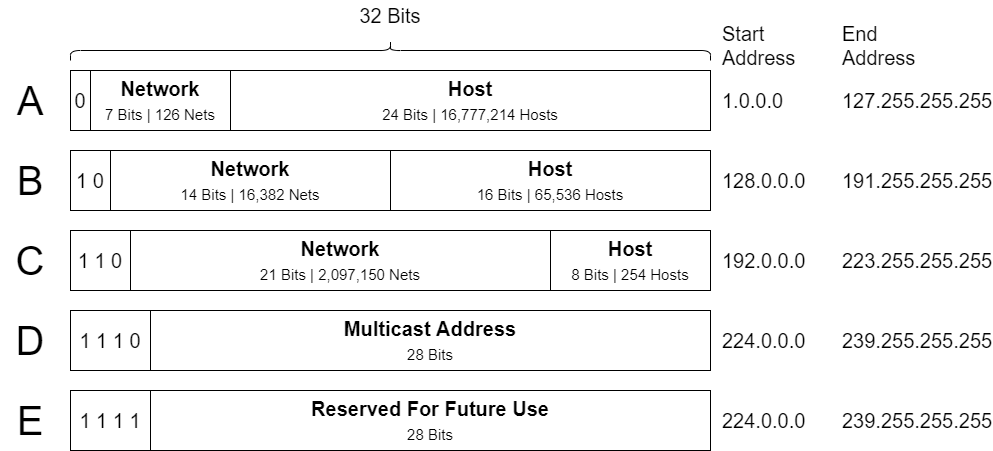
\includegraphics[width=0.8\textwidth]{network_layer/images/classful addressing.png}\end{center}
    Critical Issue: All hosts on the network must share the network address section, so if an organisation hast hosts with several different IPs, it must publicly announce/claim multiple network identifiers.
}
\termdef{Classless Addressing}{
    \begin{center}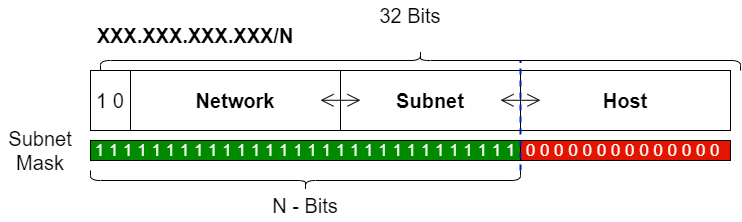
\includegraphics[width=0.8\textwidth]{network_layer/images/classless addressing.png}\end{center}
    A single network address is used for the entire organisation, internally addresses are divided into subnet addresses and host identifiers.
    \compitem{
        \item External routers only consider the network address, and forward to a router of the associated organisation.
        \item Subnet routers apply the subnet maskand check if the IP is in their subnet, or if they need to forward to another subnet in the organisation.
        \item Once a host is found, routers know which interface to forward packets to.
        \item Network, Subnet and Host can have their sizes different for each network, according to the prefix length ($N$).
        \item The any-length prefix scheme is called \textbf{CIDR} (Classless Inter-Domain Routing).
        \item Routers attempt to match the longest prefix in order to select the correct network to pass a packet onto.
    }
}
A simple python script for conversion is available with this lecture:
\codelist{Python}{network_layer/code/subnet_masks.py}
It is also covered in the lecture below:
\termdef{(DHCP) Dynamic Host Configuration Protocol}{
    Allows hosts' interfaces to safely be assigned an \textbf{IP Address}.
    \compitem{
        \item On boot, host broadcasts a \textbf{DHCP Discover} packet, a listening \textbf{DHCP} server will respond with an assigned \textbf{IP Address}.
        \item \textbf{DHCP} servers can maintain static mappings (hosts to addresses), and also assign different addresses each time a host connects.
        \item Hosts lease an \textbf{IP}, and must refresh periodically (to prevent hosts hogging an \textbf{IP}).
    }
    For example your router requests an \textbf{IP} from your \textbf{ISP}'s \textbf{DHCP} servers periodically.
}
\termdef{(NAT) Network Address Translation}{
    \begin{center}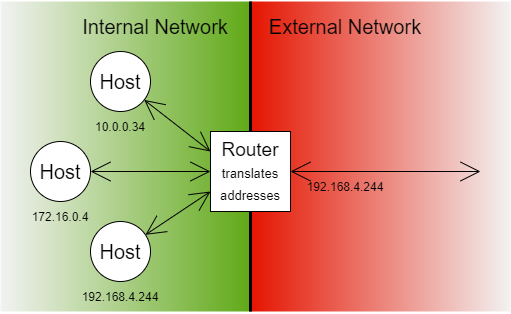
\includegraphics[width=0.6\textwidth]{network_layer/images/network address translation.png}\end{center}
    An attempt to solve the \textbf{IPv4} address shortage. Translates many private \textbf{IP}s into a single public \textbf{IP address}.
    \compitem{
        \item Translation occurs when packets leave or enter the local network.
        \item On the local/internal network, every computer gets a unique \textbf{IP address}.
    }
    This is managed with a table of mappings between hosts \& their processes (\textbf{Transport Layer}/\textbf{Layer 4} header contains this information) and ports on its own \textbf{IP}.
    \\
    \\ The following address ranges are also \textit{private} and can only be used in local networks:
    \begin{center}
        \begin{tabular}{l c l l}
            $10.0.0.0$    & $\to$ & $10.255.255.255/8$   & $16,777,216$ addresses \\
            $172.16.0.0$  & $\to$ & $172.31.255.255/12$  & $1,048,576$ addresses  \\
            $192.168.0.0$ & $\to$ & $192.168.255.255/16$ & $65,536$ addresses     \\
        \end{tabular}
    \end{center}
    There is much valid criticism of \textbf{NAT}:
    \compitem{
        \item It violates the \textbf{IP Model} (that each IP Address uniquely identifies a host).
        \item It changes the internet from connectionless to connection oriented (as router must keep track of connections, associate with a mapping for translation).
        \item It violates the fundamental rule of the protocol stack: That layers do not make assumptions about protocols above. As \textbf{NAT} uses \textbf{Transport Layer} information, if new transport protocols are used, \textbf{NAT} does not work.
        \item It cannot easily support new transport protocols (due to the previous port).
        \item Many Peer-to-Peer protocols require full connectivity between hosts which \textbf{NAT} cannot provide. Hence prot forwarding, TURN relays, NAT punching holes, 3rd party servers and other solutions are required.
    }
}
\subsubsection{Special IP Addresses}
\begin{center}
    \begin{tabular}{l p{0.7\textwidth}}
        $0.0.0.0/0$      & The \textbf{default route}, used when no other \textbf{IP address} matches.                 \\
        $0.0.0.0/8$      & This host on this interface. Must not be sent, only used to acquire an \textbf{IP Address}. \\
        $127.0.0.0/8$    & "Loopback" (reference to the host), that can be sent ($127.0.0.1$ is localhost).            \\
        $169.254.0.0/16$ & "Link Local" (something went wrong which acquiring an \textbf{IP Address}).                 \\
    \end{tabular}
\end{center}
\subsection{Ipv6}
\termdef{IPv6}{
    \begin{center}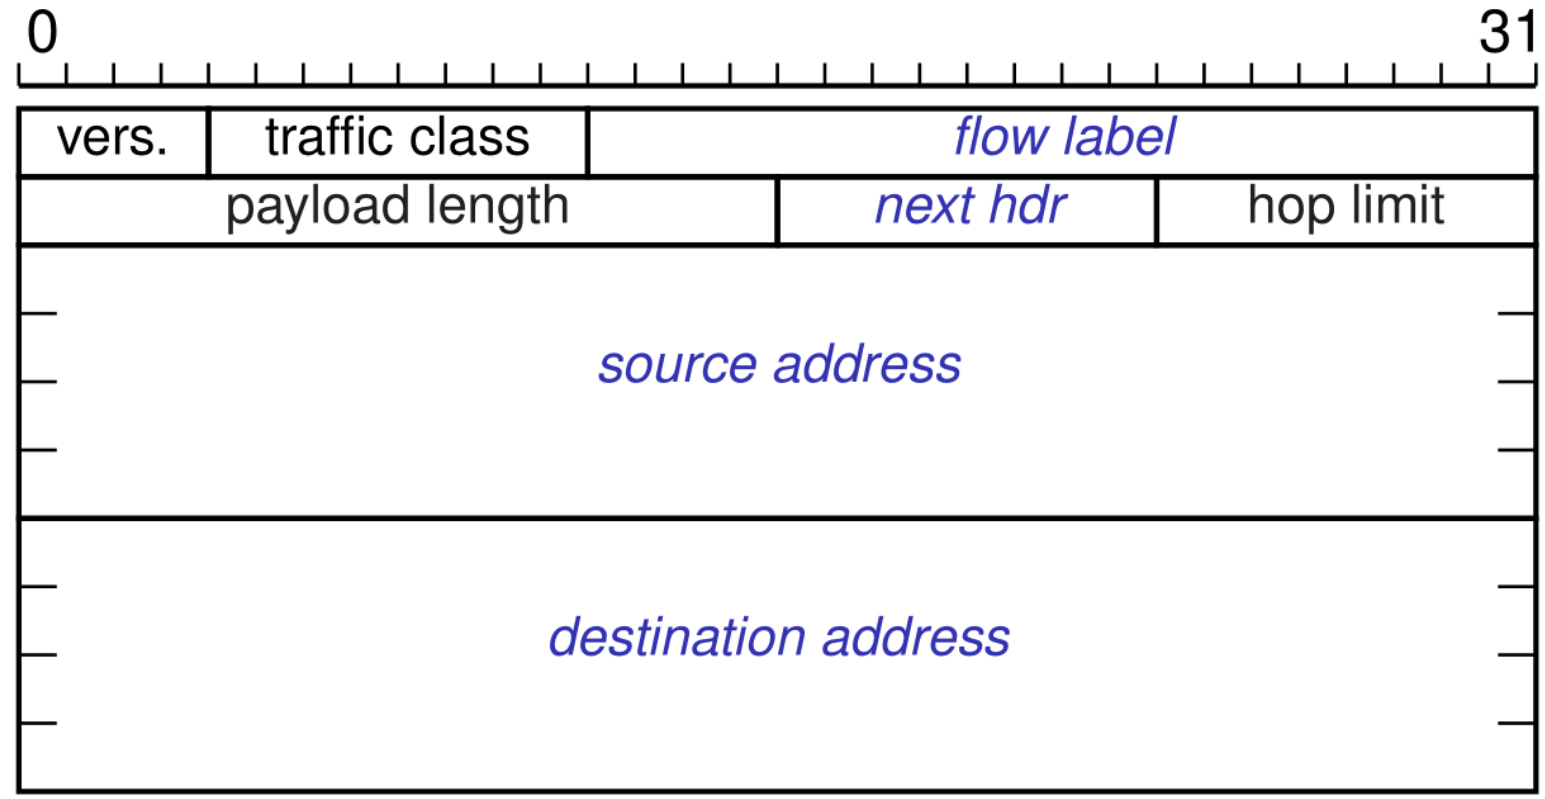
\includegraphics[width=0.6\textwidth]{network_layer/images/IPv6 header.png}\end{center}
    Intended to fix \textbf{IPv4}'s address shortage (\textbf{IPv6} has $\approx 3.8 \times 10^{38}$ addresses), while also:
    \compitem{
        \item 128 bit addresses, displayed in hexadecimal (e.g 2001:630:12:600:1:2:0:10b)
        \item Reducing routing table size and simplifying the protocol for higher performance.
        \item Improving security.
        \item Better support for "type of service" (now DiffServ in \textbf{IPv4}).
        \item Support scopes with multicasting (sending a packet to many hosts in a certain scope, e.g network).
        \item Support roaming hosts without address changes (more on roaming scopes \href{https://docs.infoblox.com/display/NAG8/About+Roaming+Hosts}{here})
        \item Better support coexistence of old and new protocols, while making it easier to develop new ones.
    }
    It has several key differences with \textbf{IPv4}:
    \compitem{
        \item Fragmentation is done by end-systems. Hence packets do not have to deal with fragmentation.
        \item No header checksum, it is redundant as both the \textbf{Transport} and \textbf{Data Link} Layers have error detection features.
        \item Fixed length header is easier to process, \textbf{IPv4}'s options were almost always unused.
        \item Better modularity for extensions.
    }
    Extensions are done by placing an extending header after the \textbf{IPv6} header.
    \compitem{
        \item Hop-by-hop options (provides information to routers, e.g quality of service)
        \item Routing (Provides a full or partial route to follow)
        \item Fragmentation (Information for end systems)
        \item Authentication (Sender identity verification)
        \item Encrypted payload (Info on the payload)
        \item Destination Options (extra information, e.g mobile \textbf{IP} (moving networks but maintaining the same IP address))
    }
}
\section{Routers}
\subsection{Routing Requirements}
A routing system needs to provide facilities for moving data from source tro destination as well as:
\compitem{
    \item Allow for multiple hops on nodes in the network.
    \item Be able to consider the topology of the network to choose appropriate routes.
    \item Perform load balancing.
    \item Allow for/deal with network heterogeneity (different types of networks connected).
}
The internet is a \textbf{packet switched} network, providing a connection-less service (no setup/teardown phase, each message is independent and self contained with no steup/tear down phase).
\\
\\ The internet is also a best effort service, and does not provide guarentees of delivery, maximum latency, bandwidth, congestion indication or in-order delivery.
\subsection{Datagram Networks}
\begin{center}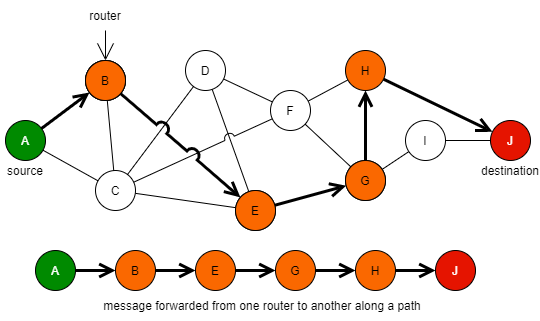
\includegraphics[width=0.8\textwidth]{network_layer/images/datagram networks}\end{center}
\compitem{
    \item There are potentially many paths for the same source to destination.
    \item Paths can be asymmetric (path from $A \to J$ is different from return path $J \to A$).
}
Each router uses a \textbf{forwarding table} to determine which router to forward packets to, based on their final destination.
\subsection{Routing}
\termdef{Sink Tree}{
    A tree from a source node, to every destination node, where each path in the tree is the optimal route/shortest path to the destination. As a tree, there are no cycles.
    \begin{center}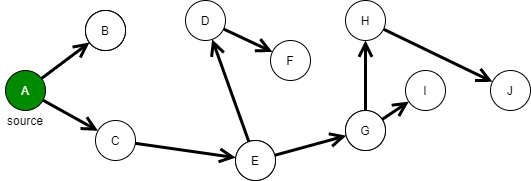
\includegraphics[width=0.7\textwidth]{network_layer/images/sink tree}\end{center}
}
\termdef{Djikstra's Algorithm}{
Each arc is labelled with a cost (e.g delay, hops, some function of parameters potentially including congestion).
\compenum {
\item Visited = $\{\}$
\item Add the start node (at $distance = 0$)
\item Loop wihile there are unvisited nodes: {
\begin{enumerate}
    \item Label each fringe node (one arc from a visited node) with the minimum of $(\text{weight from visited node}) + (\text{weight of connecting arc})$.
    \item Add the closest node (based on previous step)
\end{enumerate}
}
\item The shortest paths are the distances each node is labelled with.
}
}
Routers cooperate to find the best routes between all pairs of nodes in the network.
\termdef{Shortest Path Routing (SPR)}{
    Use \textbf{Djikstra's Algorithm} to determine the shortest routes from each router, to every destination. The forward packets accordingly.
}
\termdef{Flood Routing}{
    \begin{center}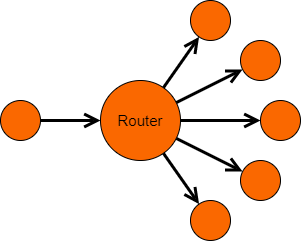
\includegraphics[width=0.3\textwidth]{network_layer/images/flood routing}\end{center}
    Forward incoming packets to every outgoing link. Except for the link the packet was received on.
    \\
    \\ We can use several strategies to avoid drowning the network in packets:
    \compitem{
        \bullpara{Hop Counter}{ Disgard a packet after it reaches a maximum number of hops.
            \\ Must decide on a correct number of hops to avoid drowining, but allow packets to reach their destination.
        }
        \bullpara{Forward Once}{ If recieving the same packet again, do not forward again.
            \\ This solves the issue where packets are sent though cycles (e.g $A \to B \to C \to A$), however it requires storing sequence numbers per source address to identify packets.
            \\ Furthermore must decide on how lonbg the sequence numbers are stored.
        }
        \bullpara{Selective Flooding}{Flood only in selective directions.
            \\ Rather than flood every outgoing link (except packet source), send to only some of the outgoing links, based on some heuristic (to decide which diurections make the most sense).
        }
    }
    Flooding always chooses the shortest path (all paths explored in parallel), however it creates significant overhead (must send many packets at every router in every path).
    \\
    \\ Use case is when the packet must be received, but when the route to the destination is unknown.
}
\termdef{Distance Vector Routing (DVR/Bellman-Ford)}{
Both \textbf{Flood Routing} and \textbf{Shortest Path Routing} are static and do not take into account current network conditions (e.g network load). \textbf{DVR} is dynamic and does consider this.
\compitem{
    \item Every router advertises its costs to each destination.
    \item Router's use their cost to neighbours, and their neighbour's cost to determine how to route packets for the minimum cost, and to then update and advertise their cost.
}
This is expressed by the \textbf{Bellman-Foprd Equation} for the cost from node $u$ to node $v$:
\[D_u'[v] = \min_{x \in neighbours(u)}(cost(u,x) + D_x[v])\]
(Cost from $u$ to $v$ is the minimum of the cost from $u$ to a neighbour, plus the cost of that neighbour to $v$)
\begin{center}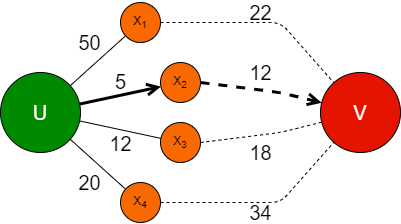
\includegraphics[width=0.6\textwidth]{network_layer/images/distance vector routing}\end{center}
However there is a \textbf{count-to-infinity} problem. When a node goes down, and routers continually update their costs based off eachothers, resulting in the cost incrementing constantly.
\[\begin{split}
        A \to C &= B \to C + 1 \\
        B \to C &= A \to C + 1 \\
    \end{split}\]
We can resolve this by defining infinite cost as:
\[cost \ \infty = \text{longest acceptable path} + 1\]
Examples of distance vector algorithms include \textbf{RIP}.
}
\termdef{Link State Routing}{
    A replacement for \textbf{DVR}.
    \compitem{
        \item Broadcasts alll information on network topology to all rputers.
        \item Each router can use this to calculate a \textbf{sink tree}.
        \item Identifies neighbours using a special "hello" packet, to which neighbours respond with their network address.
        \item Link costs is determined using a special "echo" packet, and measuring the \textbf{rount trip delay}.
    }

    The basic algorithm for each router is as follows:
    \compenum {
        \item Get direct neighbours \& their network addresses (so they are uniquely identifiable on the network) ("hello").
        \item Calculate the cost of sending packet to each neighbour ("echo").
        \item Build a \textbf{Link State Advertisement/LSA} describing the router, its connections to its neighbours.
        \item Send the \textbf{LSA} packet to every router on the network (\textbf{flooding}).
        \item Recieve \textbf{LSA} packets from every other router on the network.
        \item Now the router has the status of all links between all routers, it runs dijkstra's algorithm locally, to create a \textbf{sink tree} for use in routing.
    }
    This algorithm allows better routes to be chosen using current network conditions.
    \\
    \\ However routers may redirect traffic towards the best routes so much, that these routes become overloaded, and are no longer the best routes.
    \\
    \\ An example of \textbf{Link State Routing} is \textbf{OSPF}.
}
We can compare \textbf{DVR} and \textbf{Link State Routing}:
\begin{center}
    \begin{tabular}{l | l l}
                                 & \textbf{Distance Vector Routing}      & \textbf{Link State Routing}                          \\
        \hline
        \textbf{Network Info}    & Local                                 & Global                                               \\
        \textbf{Computation}     & Global                                & Local                                                \\
        \textbf{Synchronisation} & Gradual (routers update \& advertise) & Instance (once the \textbf{SPR} computation is done) \\
    \end{tabular}
\end{center}
\termdef{Heriarchical Routing}{
    All the previous routing methods are difficult to scale as each router needs to know about all other routers. On the scale of the internet, memory and processing power requirements would be too high.
    \\
    \\ To solve this the network is split into regions. With different algorithms used for \textbf{intra-region} (inside regions) and \textbf{inter-region} (between region) routing.
    \compitem {
        \item Can scale the network massively.
        \item Suboptimal routes chosen between node in different regions, (we just know which region to go to)
        \item Can use other algorithms within the regions, each group can effectively been its own, autonomous network with its own design, structure, routing algorithms.
        \item $2/3$ levels of regions are generally enough.
    }
    \begin{center}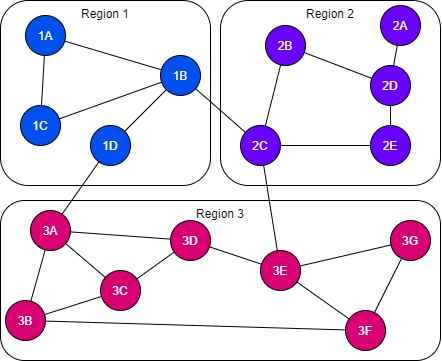
\includegraphics[width=0.7\textwidth]{network_layer/images/hierarchical routing}\end{center}
    We can consider each region a different network, all connected together.
}
\termdef{Broadcast Routing}{
    Another way to solve scaling, send to every host on a network (only feasable for \textbf{LAN}s and small \textbf{WAN}s), even through we do not know the route to a destination, by sending the packet to every host, it is sure to be recieved.
    \compitem{
        \bullpara{Send packets individually}{Not efficient}
        \bullpara{Flood Routing}{Acceptable if the flood can be limited}
        \bullpara{Multi Destination}{
            \\ A list of destinations is sent with the packet. Routers check this list, splitting the list and forwarding the packet to its neighbours.
            \\
            \\ However the packet must contain all destinations (size limitations).
        }
        \bullpara{Multicast Routing}{
            See definition.
        }
    }
}
\termdef{Reverse-Path Forwarding (RPF)}{
    Used to construct spanning trees from a router, for a low cost.
    \compitem{
        \item Every router forwards/broadcasts a packet on every adjacent router, except the router the packet was recieved from (like \textbf{flooding}).
        \item Routers only accept packets if it is on a direct path from the source.
        \item Hence the paths of packets forwarded, and accepted represents a spanning tree from the source router.
        \item Note: This can also be used to detect and prevent IP spoofing (as packet will come from an odd path, given the spoofed IP)
    }
    \begin{center}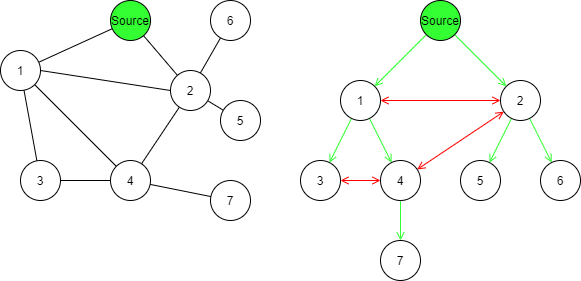
\includegraphics[width=0.7\textwidth]{network_layer/images/reverse path forwarding}\end{center}

}
\termdef{Multicast Routing}{
    Sending a message to a subset of the nodes (groups, each with a group id).
    \\
    \\ A first solution is to construct a spanning tree at each router, and prune all paths that do not contain members of the group we want to send to.
    \\
    \\ Alternatively we can use \textbf{Core based trees}.
    \compitem{
        \item A single spanning tree per group, with a root (central to the group to reduce cost between it and members of the group).
        \item To send a multicast message to the group, just send it to the core, which will retransmit to all nodes in the group.
        \item Not optimal for all sources, however scalable and much lower overhead.
    }
    Note this is how it is done in the internet (multicast IP Address/Broadcast Address is effectively the core for an entire network).
}
\section{Inter-AS Routing}
\begin{center}
    \begin{tabular}{p{0.5\textwidth} | p{0.5\textwidth}}
        \textbf{Inter-AS Routing}                                                 & \textbf{Intra-AS Routing}                                                                                 \\
        \hline
        Routing between autonomous systems (e.g between two different networks)   & Routing within an autonomous system (e.g within a \textbf{LAN}).                                          \\
        \\
        Autonomous systems can be hetergeneous (different protocols, routing algorithms, topologies, hardware) so use \textbf{Gateways} to link between.
                                                                                  & Within an autonomous system (depending on size) typically uses one design controlled by one organisation. \\
        \\
        Cannot support optimal routes at scale, but makes best attempt practical. & Attempts to provide optimal routes on a smaller network.                                                  \\
    \end{tabular}
\end{center}
\begin{center}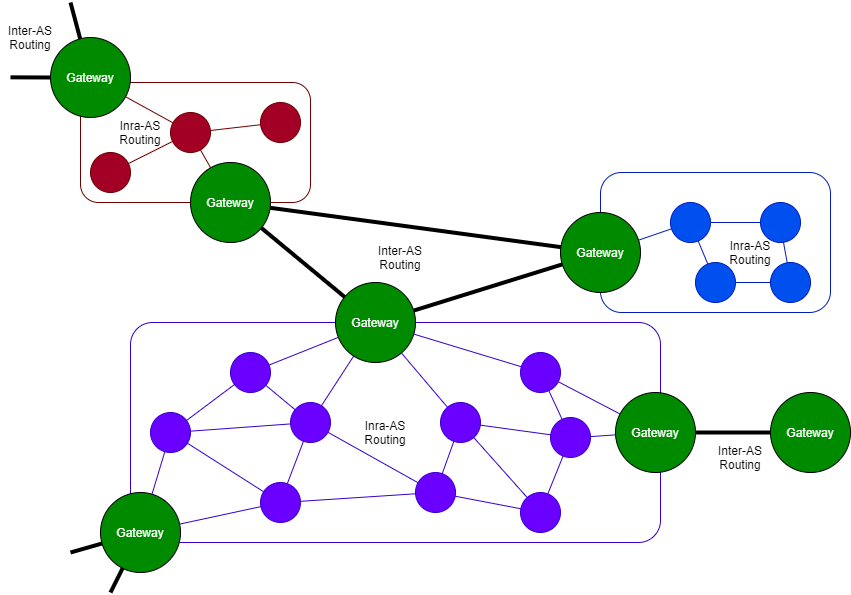
\includegraphics[width=0.9\textwidth]{network_layer/images/intra-as routing}\end{center}
\begin{center}
    \begin{tabular}{l p{0.8\textwidth}}
        $External \to External$ & Gateway (Inter-as router) recieves packet, if it can forward to the next gateway it does, if another gateway in its AS can send it, the packet is routed by intra-as routers through the network to the gateway to send on. \\
        $External \to Internal$ & Gateway recieves the packet, then sends it on to intra-as routers to route to the destination.                                                                                                                              \\
        $Internal \to external$ & Intra-as router sends packet on to a gateway that advertises it can reach the destination, gateway then forwards to the relevant gateway, routing across networks.                                                          \\
        $Internal \to Internal$ & Intra-as routers route packets.                                                                                                                                                                                             \\
    \end{tabular}
\end{center}
\termdef{Open Shortest Path First (OSPF)}{
    A \textbf{link state routing} algorithm to replace \textbf{RIP} (a distance vector routing algorithm).
    \compitem{
        \item Algorithm is publically available for anyone to implement.
        \item Supports different distance metrics (hops, delays, etc).
        \item Can adapt dynamically to changing network topology (nodes added or removed).
        \item Supports routing based on \textbf{ToS} (Type of service).
        \item Supports load balancing (not overwhelming routers e.g by flooding)
        \item Offers some security features (though some have been compromised).
    }
    It also supports hierarchical routing. It is possible to split an AS into several "areas", then each area has one or more "area border routers" which are in a "backbone area" (contains all border routers) to route traffic between the "areas".
}
\termdef{Border Gateway Protocol (BGP)}{
    The Inter-AS routing protocol used in the Internet.
    \compitem{
        \item Adjacent routers maintain connections for reliability.
        \item Gateways transmit reachability information to routers inside an AS.
        \item Good routes determined based on reachability information and routing policies.
        \item Routers only check for \& discover new paths if allowed.
        \item Uses a \textbf{path-vector} protocol (based on \textbf{DVR} but paths instead of distances are announced).
    }
    \textbf{BGP} advertises routes/paths to networks:
    \compitem{
        \item Destinations are denoted using the address prefixes (see subnetting).
        \item ASes may not propagate an advertisement by a gateway, as doing so would imply the network is willing to carry traffic through the AS.
        \item Routers can aggregate prefixes (merge prefixes together)
    }
    \example{Aggregating Prefixes}{
        We can merge several ips (with prefixes) into one, with a shorter subnet mask.
        \[\left.\begin{matrix}
                127.134.126.0/24 \\
                127.134.127.0/24 \\
            \end{matrix}\right\} \to 127.134.126.0/23 \]
        Here the 24th bit is the only difference between the two, and hence we can reduce the subnet mask size.
        \\
        \\ This is also referred to as \textit{supernetting}.
    }
    In \textbf{BGP} each AS has a unique identifier (\textbf{Autonomous System Number} (\textbf{ASN})) and several attributes:
    \compitem{
        \bullpara{AS-PATH}{Sequence of AS identifiers through which the advertisement was sent}
        \bullpara{NEXT-HOP}{Next IP address to forward packets towards advertised destination (resolves ambiguity when there are multiple AS reachable through multiple inferfaces)}
    }
    The \textbf{BGP} import policy determines to accept or reject route advertisements.
    \\
    \\ Router preference is ranked according to:
    \compitem{
        \item Policy used.
        \item Shortest \textbf{AS-PATH}
        \item closest \textbf{NEXT-HOP} router.
    }
    The \textit{count-to-infinity} problem is solved by \textit{path exploration/hunting} (actively seeks paths), furthermore routers can send withdrawal messages (e.g before taking a node down, can tell others to remove the path).
    \\
    \\ This allows routers to identify invalid paths, at the expense of some delays.
}
